% E6 / E7 results -- EmbodiedMAE-4M, yongyun branch, status as of 2026-09-22.
% Mirrors the "E6 / E7 on the yongyun branch" section of CLAUDE.md.
% Build: pdflatex E6_E7_yongyun_2026-09-22.tex   (or: tectonic ...)
\documentclass[10pt]{article}
\usepackage[letterpaper,margin=0.8in]{geometry}
\usepackage[T1]{fontenc}
\usepackage{lmodern}
\usepackage{booktabs}
\usepackage{array}
\usepackage{tabularx}
\usepackage[table]{xcolor}
\usepackage{enumitem}
\usepackage{hyperref}
\usepackage{fancyhdr}
\usepackage{caption}
\usepackage{graphicx}

\definecolor{accent}{HTML}{0B5CAD}
\definecolor{muted}{HTML}{57606A}
\definecolor{shade}{HTML}{F3F6F9}
\hypersetup{colorlinks=true,linkcolor=accent,urlcolor=accent}
\captionsetup{font=small,labelfont=bf,skip=4pt}

\newcommand{\run}[1]{\texttt{\detokenize{#1}}}
\newcommand{\key}[1]{\texttt{\detokenize{#1}}}
\newcommand{\best}[1]{\textbf{#1}}
\newcommand{\note}[1]{\par\smallskip{\footnotesize\color{muted}#1}\par}
\setlist[itemize]{leftmargin=1.2em,itemsep=2pt,topsep=3pt}
\renewcommand{\arraystretch}{1.15}
\setlength{\tabcolsep}{4pt}
\setlength{\parindent}{0pt}
\setlength{\parskip}{5pt}
% Long monospace keys cannot hyphenate; let TeX stretch spaces instead of overrunning.
\setlength{\emergencystretch}{3em}

\pagestyle{fancy}
\fancyhf{}
\renewcommand{\headrulewidth}{0pt}
\fancyfoot[L]{\footnotesize\color{muted}EmbodiedMAE-4M $\cdot$ E6 / E7 $\cdot$ yongyun branch $\cdot$ 2026-09-22}
\fancyfoot[R]{\footnotesize\color{muted}\thepage}

\begin{document}

{\LARGE\bfseries E6 / E7 results: structured masking, noise, spline params, PC loss\par}
\vspace{3pt}
{\color{muted}EmbodiedMAE-4M, \texttt{yongyun} branch $\cdot$ status as of 2026-09-22 $\cdot$
mirrors the ``E6 / E7 on the yongyun branch'' section of \texttt{CLAUDE.md}\par}

\section*{Bottom line}
\begin{itemize}
  \item \textbf{Occlusion recipes (E6): no winner.} The four blob-size $\times$ noise recipes differ
        by about as much as the same recipe run twice with a different seed. Recipe~B
        (\key{length_scale} 0.20, $1\times$ noise) stays the default: best observed, not shown better.
  \item \textbf{The spline params already help.} With every param token visible, swapping a
        sample's own params for the val-set mean makes PC Chamfer 7\,\% worse, far above the
        0.6\,\% seed noise.
  \item \textbf{The params fix (v2 + camera pose/scale) has not worked yet.} It did not raise
        reliance on the params, and PC Chamfer got 6\,\% worse. Suspected cause: v2's param loss is
        ${\sim}6\times$ larger and takes gradient from the PC term. The next run rescales
        \key{spline_loss_weight} to ${\sim}0.6$.
  \item \textbf{The model's weak point is leaf tips, not the frame edge.} The edge-biased mask
        does mask the border more (0.64 $\to$ 0.89), but the border is background. On the plant,
        PC error on the outermost points is ${\sim}10\times$ the centre's.
  \item \textbf{PC loss study (E7): 1 of 11 arms finished.} QAL threshold 0.005 matches the 0.01
        baseline within noise. The Chamfer and Sinkhorn arms have not run yet.
\end{itemize}

\section*{Setup shared by every run}
\begin{itemize}
  \item 4M base $\cdot$ 3\,000 train plants, one randomly drawn view per plant per epoch $\cdot$
        \textbf{30\,000 optimizer steps} (94 steps/epoch $\to$ \textbf{320 epochs}) $\cdot$
        global batch 32 (8 per GPU $\times$ 4 L40S) $\cdot$ \texttt{Sorghum\_15K} split. Best
        checkpoints land at epochs 300--320: still improving when the cosine schedule ends.
  \item Clean val: a fixed 225-view subset. Occluded val: one reference corruption shared by all
        runs (\key{occlusion.}\allowbreak\key{eval_occlusion} at $1\times$ noise), so occluded numbers are comparable.
  \item \textbf{Held fixed, including the edge weighting.} Structured token masking on half the
        batches (\key{prob} 0.5) with \key{center_bias} 1.5: masked blobs gather at the frame border
        and the centre plant stays visible; train-only, so validation uses uniform masks. Procedural
        occluding leaves enter from outside the frame (\key{reach} 0.6--1.2, 9--16 leaves, every
        sample), interleaved in depth, plus sensor noise. \textbf{No run varies \key{center_bias},
        \key{prob} or \key{reach}}, so these results do not say whether the edge weighting helps.
  \item 30\,000 steps is ${\sim}15\,\%$ of the main programme's 197\,400-step budget
        (\run{e3_3k}, same 94 steps/epoch, runs 2\,100 epochs): rankings transfer, absolute numbers
        do not. The 3\,000 plants are not the same draw as main's
        \run{e3_3k}.
\end{itemize}

\section*{Noise floor: read every table against this}
Training had no seed before \key{training.seed} was added, so \run{recipe_b} (unseeded) and
\run{params_v1_seed1} (seed 1) are the same configuration run twice. Their gap is the only
run-to-run error bar available.

\begin{center}
\centering\small
\begin{tabular}{lccccccc}
\toprule
 & val loss & val (occ) loss & PC Chamfer & F1@0.01 & F1@0.03 & EMD & Depth MSE \\
\midrule
seed-to-seed gap & 0.027 & 0.014 & 0.6\,\% & 1.7\,\% & 0.3\,\% & 1.4\,\% & 11\,\% \\
\bottomrule
\end{tabular}
\captionof{table}{One pair of runs, so this is itself a rough estimate. Differences smaller than this are
treated as noise.}
\end{center}

\section*{Which F1 threshold}
F1@0.03 is the headline column: its ceiling is ${\sim}1$, so the value reads directly as a fraction
of a perfect reconstruction. F1@0.01 is kept beside it. Its ceiling is well below 1, because two
independent 8\,196-point draws of the \emph{same} ground-truth cloud only reach:

\begin{center}
\centering\small
\begin{tabular}{lcccc}
\toprule
 & F1@0.005 & F1@0.01 & F1@0.02 & F1@0.03 \\
\midrule
perfect reconstruction (sampling limit) & 0.465 & 0.871 & 0.995 & 0.999 \\
our models & -- & 0.150--0.159 & 0.403--0.416 & 0.575--0.586 \\
\bottomrule
\end{tabular}
\end{center}

So F1@0.01 = 0.154 is ${\sim}18\,\%$ of what is reachable. It is also slightly the more
discriminating column here (recipe spread / seed gap $3.1\times$ vs $2.7\times$ at 0.03), and it is the
one that exposes the leaf-tip failure below. Moving to a threshold where F1 $\approx 0.9$ would not
help: every arm saturates there and the gaps compress.

\section*{E6: structured-mask blob size $\times$ sensor noise}
\begin{center}
\centering\scriptsize
\rowcolors{2}{white}{shade}
\begin{tabular}{llccccccccc}
\toprule
 & run & blob size & train noise & val loss & val (occ) & PC Chamfer & F1@0.03 & F1@0.01 & RGB MSE & Depth MSE \\
\midrule
A  & \run{recipe_a_ls035_noise1x}   & 0.35 & $1\times$   & 0.5829 & 0.5964 & 0.004703 & 0.5832 & 0.1582 & 0.6738 & 0.03350 \\
B  & \run{recipe_b_ls020_noise1x}   & 0.20 & $1\times$   & 0.5623 & 0.5853 & 0.004644 & 0.5856 & 0.1567 & 0.6649 & 0.03355 \\
C  & \run{recipe_c_ls020_noise0p5x} & 0.20 & $0.5\times$ & 0.5908 & 0.5993 & 0.004716 & 0.5816 & 0.1536 & 0.6715 & 0.03219 \\
D  & \run{recipe_d_ls020_noise2x}   & 0.20 & $2\times$   & 0.5891 & 0.6010 & 0.004680 & 0.5817 & 0.1503 & 0.6610 & 0.03221 \\
B$'$ & \run{params_v1_seed1} (= B, seed 1) & 0.20 & $1\times$ & 0.5891 & 0.5996 & 0.004670 & 0.5841 & 0.1541 & 0.6773 & 0.02997 \\
\bottomrule
\end{tabular}
\captionof{table}{Blob size = \key{length_scale}. $1\times$ noise = rgb 0.03 / depth 0.015 / pc 0.008 (std). B$'$ is B re-run with only the random seed changed, so B vs B$'$ is the run-to-run noise. Nothing is bold: no gap in this table exceeds that seed-to-seed gap.}
\end{center}

B has the best clean and occluded val loss, but \textbf{B run a second time (B$'$) lands behind A
and level with C and D.} Every recipe gap (A$-$B 0.021, C$-$B 0.029, D$-$B 0.027 in val loss) is the
size of the seed gap, so the sweep does not rank these recipes, and the order of A and B flips with
the F1 threshold (A $>$ B at 0.01, B $>$ A at 0.02 and 0.03). Separating them needs at least three
seeds per arm.

\section*{Where the model fails: leaf tips, not the frame edge}
Trained recipe-B model, 12 val plants, 4 mask draws. Radius 0 = image centre, 1 = corner (for the PC,
the $xy$ radius of the unit-normalised cloud). Errors are on \emph{masked} patches.

\begin{center}
\centering\small
\begin{tabular}{lccccc}
\toprule
radius & 0--0.2 & 0.2--0.4 & 0.4--0.6 & 0.6--0.8 & 0.8--1 \\
\midrule
plant share of patches & 71\,\% & 40\,\% & 16\,\% & 3\,\% & 0.2\,\% \\
P(masked), uniform mask & 0.64 & 0.61 & 0.60 & 0.60 & 0.62 \\
P(masked), structured (\key{center_bias} 1.5) & 0.64 & 0.70 & 0.81 & 0.86 & 0.89 \\
RGB MSE, all masked patches & 0.18 & 0.17 & 0.09 & 0.02 & 0.002 \\
RGB MSE, plant patches only & 0.20 & 0.25 & 0.29 & 0.27 & 0.60 \\
PC: target point $\to$ nearest prediction & 0.025 & 0.042 & 0.072 & 0.119 & 0.233 \\
\bottomrule
\end{tabular}
\end{center}

The edge bias does what it says: masking rises from 0.64 to 0.89 toward the corner. But the corner
is background, which is why the error there is near zero. On the plant itself, error \emph{grows}
outward, and PC error on the outermost points is ${\sim}10\times$ the centre's: the model misses leaf
tips. That is the low F1@0.01 (precision 0.40, recall 0.11 at the end of training: predicted points
sit on the dense core and do not reach the tips). Much of the edge-biased mask budget is therefore
spent on background; masking the plant's \emph{outer parts} would target the actual failure.

\begin{center}
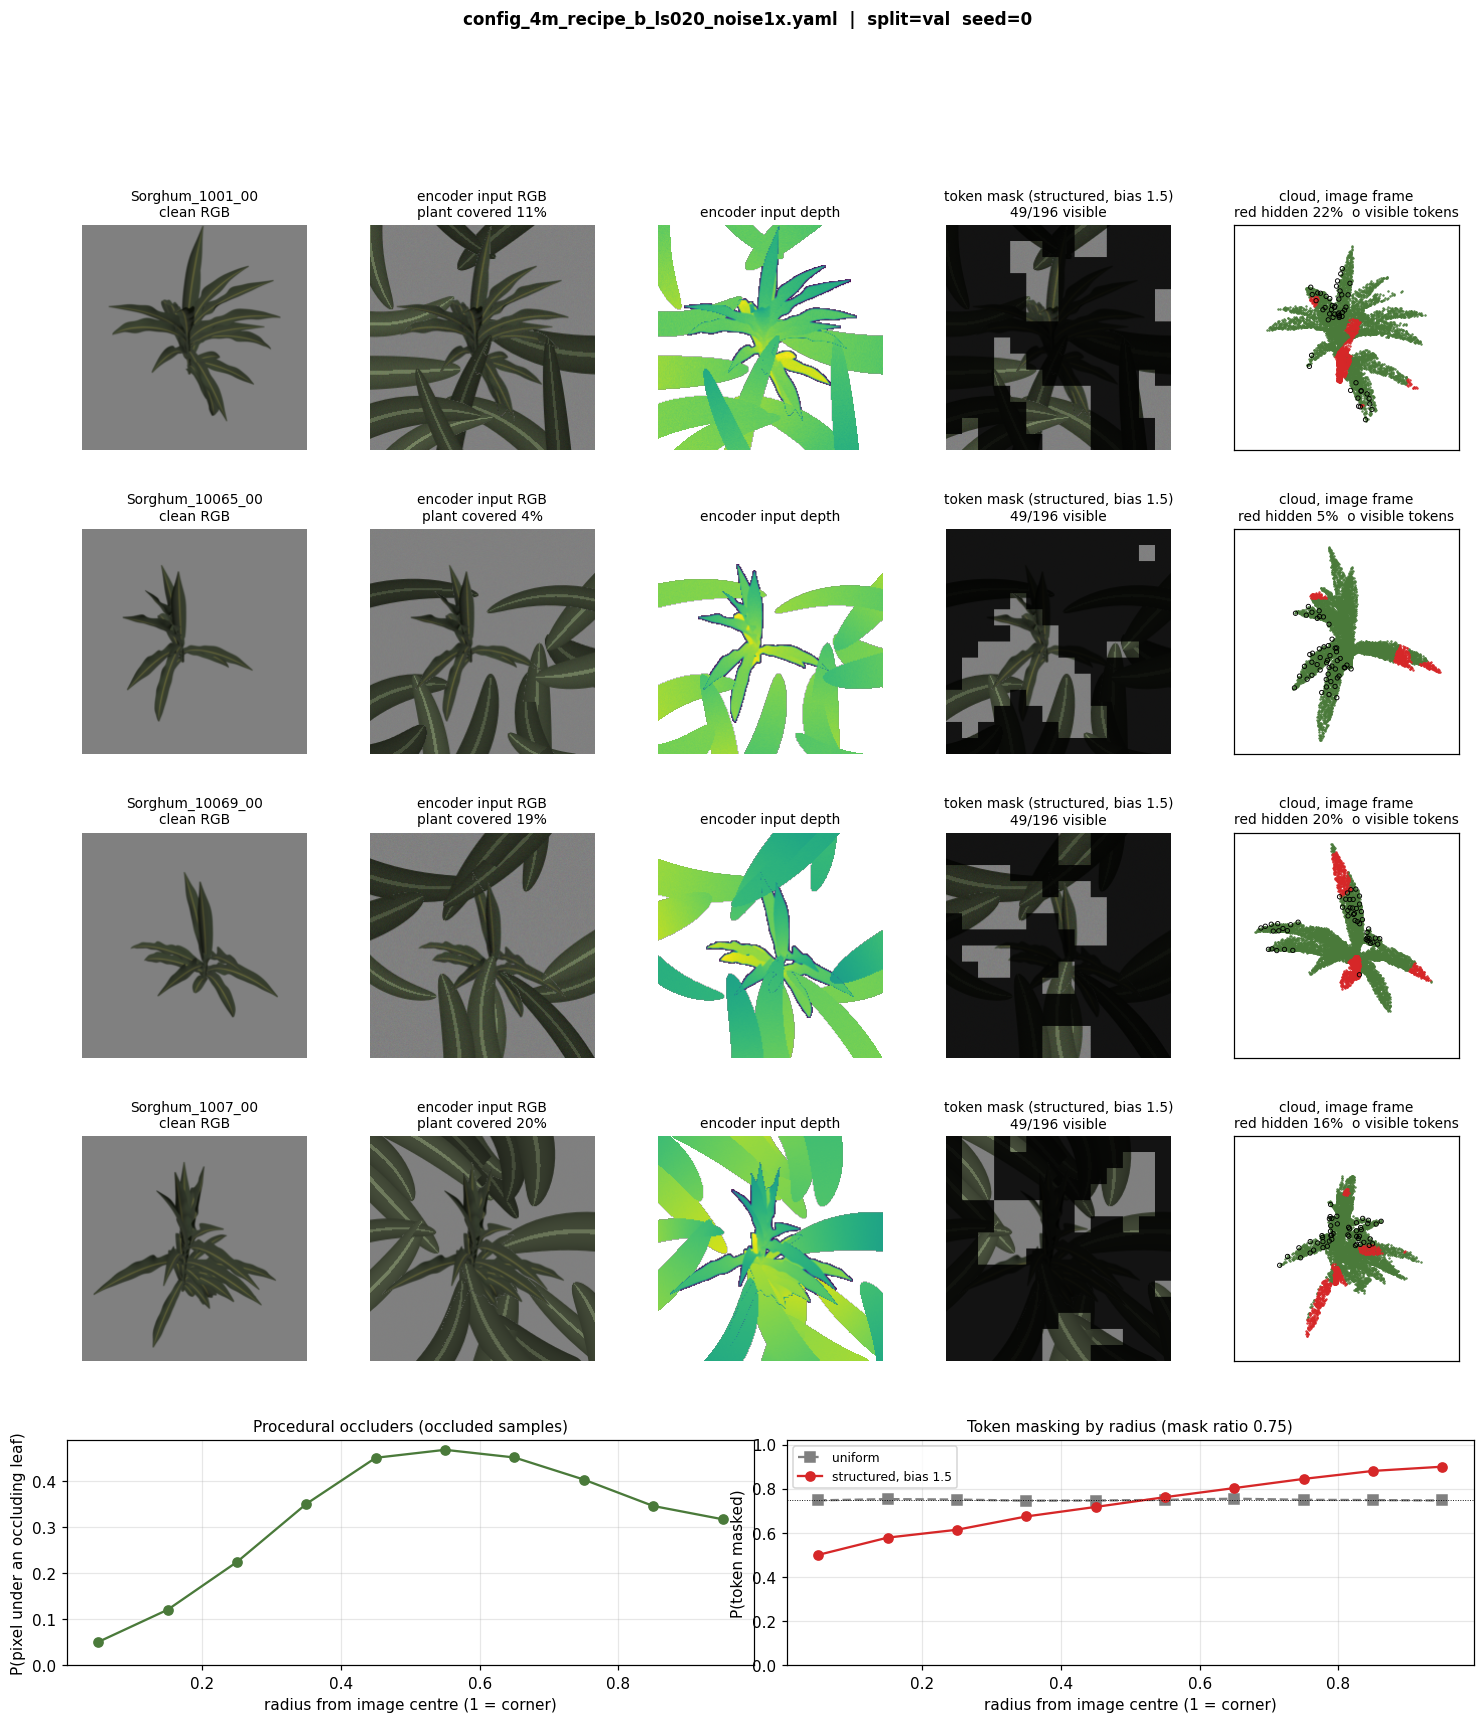
\includegraphics[width=0.85\linewidth]{mask_preview_recipe_b.png}
\captionof{figure}{Recipe-B masks on four val plants: clean RGB, occluded encoder input, depth,
structured token mask (49 of 196 tokens visible) and the PC with hidden points in red. Bottom: occluder
coverage and token-mask probability by radius.}
\end{center}

\section*{Spline params: do they help, and does fixing their encoding help more?}
Measured on the data first: 5 of the 9 plant dims (\key{panicle_*}) are constant; the per-sample PC
normalisation removes absolute size (correlation of \key{stem_length} with cloud height is 0.68 raw,
0.08 after normalisation); and the params live in the plant's world frame while the PC target is in
the camera frame, with the \key{camera_pose.json} that links them never read. \textbf{v2} z-scores
the params, encodes angles as $(\sin,\cos)$, drops the constant dims and adds the leaf count;
\textbf{geometry conditioning} feeds the camera rotation and normalisation radius as an
always-visible token. Same seed; only the params path differs.

\begin{center}
\centering\footnotesize
\begin{tabular}{lccccccc}
\toprule
run & PC Chamfer & F1@0.01 & F1@0.02 & F1@0.03 & EMD & RGB MSE & Depth MSE \\
\midrule
v1 \quad \run{params_v1_seed1}               & \best{0.004670} & 0.1541 & 0.4097 & \best{0.5841} & 0.2966 & 0.6773 & 0.02997 \\
v2 + pose/scale \quad \run{params_v2cond_seed1} & 0.004967 & \best{0.1587} & 0.4057 & 0.5748 & 0.2948 & 0.6758 & 0.03256 \\
\bottomrule
\end{tabular}
\captionof{table}{Bold = better than the other run by more than the seed-to-seed gap (PC Chamfer 0.6\,\%, F1@0.01 1.7\,\%, F1@0.03 0.3\,\%); every other gap is within noise.}
\end{center}

\textbf{Oracle test} (\run{eval_param_oracle.py}): all param tokens visible; the sample's own params
vs the val-set mean, with identical RGB / depth / PC masks in both passes. Positive = worse without
the sample's own params, i.e.\ the params are being used.

\begin{center}
\centering\small
\begin{tabular}{lcccccc}
\toprule
checkpoint & PC Chamfer & F1@0.01 & F1@0.02 & RGB MSE & Depth MSE & occluded PC Chamfer \\
\midrule
v1              & $+7.0\,\%$ & $+1.4\,\%$ & $+2.1\,\%$ & $-1.7\,\%$ & $+7.1\,\%$ & $+7.9\,\%$ \\
v2 + pose/scale & $+4.6\,\%$ & $+5.3\,\%$ & $+2.5\,\%$ & $+0.4\,\%$ & $-0.2\,\%$ & $+4.5\,\%$ \\
\bottomrule
\end{tabular}
\end{center}

\textbf{The params already help in v1.} v2 + pose/scale did not increase that reliance, and its
absolute PC Chamfer is 6\,\% worse. Most likely cause, not yet isolated: v2's Smooth-L1 targets are
z-scores, so the param loss is ${\sim}6\times$ v1's at the same \key{spline_loss_weight} of 5.
Next: v2 with \key{spline_loss_weight} $\approx 0.6$; if still flat, asymmetric masking (steps with the
PC fully masked and the params fully visible).

\section*{E7: point-cloud loss study (in progress)}
Weights were set from loss magnitudes measured on the trained recipe-B model: QAL 0.060, Chamfer
0.0053 ($11\times$ smaller), Sinkhorn $\approx 0.055$. Chamfer therefore needs \key{pc_loss_weight}
$\approx 10$ to pull as hard as QAL at 1. ``Sinkhorn only'' is a new option
(\key{loss_name}: \key{sinkhorn}, on 2\,048 sampled points); before, Sinkhorn existed only as an auxiliary
term. Everything else matches \run{params_v1_seed1}, which serves as the QAL baseline arm.

\begin{center}
\centering\footnotesize
\begin{tabularx}{\linewidth}{l >{\raggedright\arraybackslash}X >{\raggedright\arraybackslash}X l}
\toprule
loss & settings & runs & status \\
\midrule
QAL & threshold 0.005 / 0.01 / 0.02 at $\alpha=100$; $\alpha$ = 30 / 300 at threshold 0.01
    & \run{loss_q_t005}, \run{params_v1_seed1}, \run{loss_q_t020}, \run{loss_q_a030}, \run{loss_q_a300}
    & 2 done, 1 running, 2 queued \\
Chamfer & \key{pc_loss_weight} 3 / 10 / 30 & \run{loss_c_w03}, \run{loss_c_w10}, \run{loss_c_w30} & queued \\
Sinkhorn only & blur 0.01 / 0.02 / 0.05 at weight 1; blur 0.02 at weight 3
    & \run{loss_s_b010_w1}, \run{loss_s_b020_w1}, \run{loss_s_b050_w1}, \run{loss_s_b020_w3} & queued \\
\bottomrule
\end{tabularx}
\end{center}

Finished so far, compared only on metrics computed identically for every arm (val loss is a
different quantity per loss):

\begin{center}
\centering\footnotesize
\begin{tabular}{llccccccc}
\toprule
run & setting & PC Chamfer & F1@0.01 & F1@0.02 & F1@0.03 & EMD & RGB MSE & Depth MSE \\
\midrule
\run{params_v1_seed1} & QAL $t=0.01$, $\alpha=100$  & 0.004670 & 0.1541 & 0.4097 & 0.5841 & 0.2966 & 0.6773 & 0.02997 \\
\run{loss_q_t005}     & QAL $t=0.005$, $\alpha=100$ & 0.004700 & 0.1540 & 0.4060 & 0.5822 & 0.2970 & 0.6910 & 0.02898 \\
\bottomrule
\end{tabular}
\captionof{table}{Halving the QAL threshold moves nothing past the noise floor.}
\end{center}

Progress: the \texttt{mech-ai} account is at its 17-GPU cap, so the arms run one at a time
(${\sim}5$\,h each, 4 GPUs per arm). At that pace the last arm finishes around Sep~24.
Full table: \texttt{python compare\_recipes.py --loss-study}.

\section*{Before merging with main}
\begin{itemize}
  \item New config keys, all off by default (with none set, a model is bit-identical to before):
        \key{training.}\allowbreak\key{num_train_plants}, \key{views_per_epoch},\allowbreak\ \key{max_steps}, \key{seed};
        \key{occlusion.}\allowbreak\key{eval_occlusion}; \key{model.}\allowbreak\key{param_encoding}, \key{geometry_cond};
        \key{loss_name}: \key{sinkhorn}.
  \item Main implements plant subsetting and view sampling separately (\key{data.max_plants},
        \key{data.view_sampling}). Keep one when merging; they will conflict in
        \run{train_sorghum_4m.py} and the datasets.
\end{itemize}

\end{document}
